\documentclass[10pt]{article}
\usepackage{amsfonts}
\usepackage{amsmath}
\usepackage[font=small,labelfont=bf]{caption}
\usepackage{fancyhdr}
\usepackage[margin=1.0in]{geometry}
\usepackage{graphicx}
\usepackage{hyperref}
\usepackage{multicol}
\usepackage{textcomp}
\newcommand\floor[1]{\lfloor#1\rfloor}
\newcommand\ceil[1]{\lceil#1\rceil}
\setlength{\columnsep}{0.5cm}
\setlength{\headheight}{24pt}
\setlength{\parindent}{15pt}
\pagestyle{fancy}
\fancyhf{}
\lhead{
	CSE 847: Machine Learning---Final Report \\
	Langford, Lingg, and Lucero
}
\rhead{April 28, 2017}
\cfoot{\thepage}
\begin{document}
	\title{
		CSE 847: Machine Learning---Final Report \\
		\textbf{An Exploration and Implementation of Automated Valuation Models to Learn and Predict the Value of Real Estate}
	}
	\author{
		\begin{tabular}{ccc}
			Mick Langford & Mike Lingg  & Jordi Lucero \\
			langfo37@msu.edu & linggmic@egr.msu.edu & luceroj2@msu.edu \\
			\textit{Neural Network} & \textit{Linear/Logistic Regression} & \textit{Decision Trees}
		\end{tabular}
	}
	\date{April 28, 2017}
	\maketitle
	\begin{multicols}{2}
		\section{Problem Description}
		Automated Valuation Models (AVM) have become increasingly popular as the real estate market has embraced the World Wide Web as a source of accurate, up to the minute data.\textsuperscript{\cite{kaggleblog}} Banks have also shown great interest in using AVMs to help mitigate fraud by human appraisal.\textsuperscript{\cite{scotsman}} Our goal is to explore various machine learning techniques to implement an AVM and predict the true value of a house based on features commonly found on real estate listings. Our data will be drawn from various datasets, including from the Nashville, TN housing market, using a dataset posted on Kaggle\textsuperscript{\cite{nashville_data}}.
		
		We have implemented both linear and logistic regression models that take into account physical attributes of each house and location. We have also implemented nonlinear models, such as decision trees and neural networks for comparison.

		The work in this projection was split between the three team members most based on the implementation approach. Mike Lingg implemented the Linear and Logistic Regression techniques discussed in sections 5.1 and 5.3, and much of the pre-processing work described Section 4. Mick Langford did most of the data gathering for related works and implemented the Neural Network described in Section 5.5. Jordi Lucero implemented the Decision Tree models described in Section 5.4.
		
		\section{Related Work}
		An obvious and popular example is Zillow's proprietary Zestimate\textsuperscript{\textregistered}. Zillow uses a closed source AVM that takes into account special features of the home, location, and market conditions. Zillow admits to using features such as physical attributes, tax assessments, and prior transactions. Zillow claims to have data on 110 million homes and estimates on approximately 100 million homes.\textsuperscript{\cite{zillow}}

		Relevant papers include the doctoral dissertation of Lowrance which explores and compares various linear models on housing data for the Los Angeles County.\textsuperscript{\cite{lowrance}} Park and Bae explore machine learning algorithms such as C4.5, RIPPER, Naive Bayesian, and AdaBoost.\textsuperscript{\cite{park}} Bin performed a study that estimates a hedonic price function using a semi-parametric regression.\textsuperscript{\cite{bin}} This may be particularly useful for real estate listings that are incomplete or for data that is entered erroneously. Bourassa et al. consider the spatial dependence of house prices, which is intuitively an important factor.\textsuperscript{\cite{bourassa1}\cite{bourassa2}} Kauko et al. research neural network models to help investigate segmentation in the housing market of Helsinki, 
		
		Finland.\textsuperscript{\cite{kauko}} Azadeh et al. present an algorithm based on fuzzy linear regression and a fuzzy cognitive map to handle uncertainty in the housing market and improve the analysis of housing price fluctuations.\textsuperscript{\cite{azadeh}} Fan et al. introduce a decision tree approach for modeling and predicting house prices.\textsuperscript{\cite{fan}}

		\section{Project Data}
		Multiple sources of real housing sales data are considered for this project:

		\textbf{Nashville}. The Nashville housing dataset is a list of home sales in the Nashville, Tennessee area, provided by Kaggle\textsuperscript{\cite{nashville_data}}. This dataset includes 29 fields of data for 56635 entries. However, nearly half of the entries have gaps in information, which will have to be accounted for.

		\textbf{King County}. The King County housing dataset is a list of home sales in the King County, Washington area, provided by Kaggle\textsuperscript{\cite{kc_data}}. This dataset includes 20 fields of data for 21614 entries, with none of the entries missing any data.
		\par
		\textbf{Advanced Regression Techniques (ART)}. The Advanced Regression Techniques data is a list of home sales, provided by Kaggle. This data includes 79 features of housing data for 1460 homes. The data has no gaps, except for some N/A data.
		\par
		\textbf{Grand Rapids}. The Grand Rapids data is a list of home sales in the Grand Rapids area, provided by the real estate listing service Redfin. This data includes 16 fields for 9646 entries. The dataset also has gaps in information for about half of the entries.
		\par
		The different datasets provide a variety of input to test machine learning techniques against. Data with more features should provide more accurate results, if the additional features provide useful information for the prediction.
		
		\section{Preprocessing Data}
		Prior to processing the data with our models, each dataset is first normalized by dividing each feature value by the difference between that feature's maximum and minimum values. The target sales prices are normalized across all datasets to allow for comparison of the model's performance. One issue considered is how to properly manage fields containing categorical values. Our approach is to treat a field with \(n\) categories as \(n\) binary features, indicating whether that entry is of the associated category or not. Finally, since some of our datasets are incomplete, different methods of substituting missing values are considered, such as using the feature mean, substituting values from the closest neighbor by way of Euclidean distance, or using the mean value from a group of closest neighbors.

        Table \ref{table:linr_preprocessing} shows the results of data preprocessing with a simple closed form linear regression, using the ART Data. First, the data is considered with no preprocessing, with exception to the sale prices, which are normalized so that Mean Squared Error (MSE) can be compared between the results. Second, both the features and home prices are normalized. Third, in addition to normalization, all categorical features are split into a number of binary features for each categorical value. The observed results confirm that each additional method of preprocessing improves the MSE significantly. As a result of this analysis, the decision was made to preprocess all of our data by normalizing the values and splitting categorical features into binary.
        
		Basic closed form linear regression cannot be solved without either discarding entries with missing values or using some method of substitution. Table \ref{table:linr_hole_fill} provides a comparison of the methods considered for replacing missing values. These results are from applying closed form linear regression to the Grand Rapids dataset from Redfin. Using the mean value of the missing features is a valid option but is not ideal. To improve upon this, each member in the set of incomplete entries is compared to those that are complete, computing the Euclidean distance between the known values of each incomplete entry. The corresponding values in the nearest complete entry to each incomplete entry is used as a substitute. This method demonstrated an improvement in observed MSE from linear regression. However, an even greater improvement is found when instead of just using the values from the closest neighbor to each incomplete entry, the mean values from the ten closest neighbors is used instead. This final method of substitution should be assumed for all of the models discussed in this report.
		\begin{center}
			\captionsetup{type=table}
			\begin{tabular}{l|c}
				Feature Preprocessing 	& MSE \\
				\hline
				None 					& 1.2487 \\
				Normalization 			& 0.0499 \\
				Binary Features 		& 0.0012 \\
			\end{tabular}
			\captionof{table}{MSE for preprocessing techniques.}
			\label{table:linr_preprocessing}			
		\end{center}

		\begin{center}
        	\captionsetup{type=table}
			\begin{tabular}{l|c}
				Substitution Method & MSE \\
				\hline
				None 				& ---\\
				Mean 				& 1.6e-3 \\
				Closest Value 		& 1.2e-3 \\
				Closest Mean 		& 1.1e-3 \\
			\end{tabular}
			\captionof{table}{MSE for missing value substitution.}
			\label{table:linr_hole_fill}
		\end{center}

        During the course of research, the MSE measured by our models was observed to be producing greatly different results between datasets. Models that appeared to produce a good match were resulting in higher error than models that appeared to produce weaker results. It was observed that the datasets producing lower error had more lower-valued houses and few high-valued. This issue was addressed by filtering out any homes with sales prices above \$1M, in order to eliminate these boundary cases. Outliers were pruned prior to missing value substitution, to ensure that the pruned entries has no influence on substituted values. Additionally, the target sales prices were normalized across all datasets to ensure that the MSE computed by each model for each dataset could be compared.
        
 		\section{Models}
		\subsection{Linear Regression}
		For linear regression we are using a closed form ridge regression. We tested standard and stochastic gradient descent but these methods did not produce a significant improvement in processing time for the data we are using, and do not improve on the prediction error.

		For the ridge regression regularization value we developed a simple automated approach to identify the ideal regularization value. We start with a test regularization value of 1 and perform five fold cross validation on the training data to determine the mean square error with this test value. Then we adjust the test value by 0.1 in the positive direction, in this case moving from 1 to 1.1, and repeat the cross validation. If the error decreases, we continue to adjust the test value in the same way. If the error increases, we reverse the sign of the test value adjustment and divide it by 10. This is like a simplistic gradient descent, but when we overshoot the minimum we reverse direction and lower the step size. This continues until the error between two cross validations matches within 1e-7.

		\begin{center}
            \captionsetup{type=figure}
			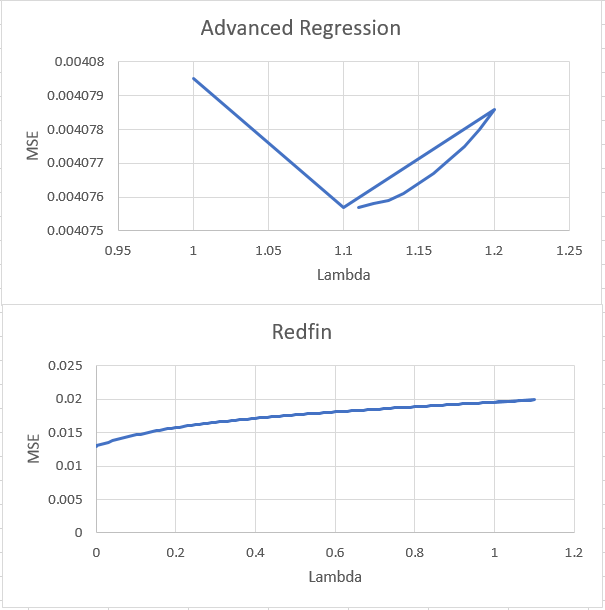
\includegraphics[scale=0.60]{Images/LinearRegressionCrossTrain} \\
			\captionof{figure}{Linear regression cross training.}
			\label{fig:linr_cross_train}
		\end{center}

        Figure \ref{fig:linr_cross_train} shows a sample of our cross training method on the ART and Grand Rapids datasets. The advanced regression data initially shows a reduced error when moving from 1 to 1.1 so it increases to 1.2.  At 1.2 the error goes back up again so it reverses direction and moves back in increments of 0.01, until it reaches a stable point. This shows a place where the algorithm works but could possibly have been made more efficient, but still works for our current purposes. The Grand Rapids data starts at a regularization value of 1 but sees an increase of error at 1.1 so decreases at a lower rate. What can be seen in the data, but is not visible in the graph, is around 0.013 lambda the regularization search reverse direction, an dincreases precision, several times to find the minimum solution.

		Table \ref{table:linr_performance} shows the mean square error of linear regression for each dataset. As expected the advanced regression techniques dataset provides the least error as this data provides the most complete features for each house. Nashville performs the weakest as there are very large gaps in the data, which must be filled in by preprocessing. The interesting result is between Grand Rapids and King County data. The King County dataset has the same number of features as the Grand Rapids Data and more homes in the dataset. Preprocessing the data shows that the redfin features have more categories and the redfin house prices are concentrated more at the lower end, whereas the King County features have few categories and have prices fairly evenly distributed over the normalized range. As a result, redfin has more information in the features and the prices are easier to predict, which appears to be what produces the lower error.

		\begin{center}
      	\captionsetup{type=table}
			\begin{tabular}{l|c}
				Dataset			& MSE \\
				\hline
				Nashville 		& 22.1e-3 \\
				ART 			& 1.0e-3 \\
				King County 	& 13.1e-3 \\
				Grand Rapids 	& 6.3e-3 \\
			\end{tabular}
			\captionof{table}{Observations from linear regression model.}
			\label{table:linr_performance}        
		\end{center}
	
		We also tried two ensemble methods with linear regression. The first method divides the features into groups of 4, performs linear regression on each group and adds the group results together. Linear regression is then performed on the summation of the groups. The second method picks random groups of 10 features with 100 groups and then an ensemble is produced in the same method as the groups of 4 in the previous method. Additionally each ensemble method was tested with PCA feature reduction providing 25\%, 50\%, 75\% and 100\% of features. This method was tested against all of the datasets except for the Nashville data as an SVM on the Nashville data exceeded matlab's available memory.

        Figure \ref{fig:linr_ensemble} shows the results of the ensemble methods. The advanced regression techniques and King County data performed close to the pure linear regression. The redfin dataset showed a slight improvement over linear regression.

		\begin{center}
            \captionsetup{type=figure}
			\includegraphics[scale=0.6]{Images/LineEnsembleResults} \\
			\captionof{figure}{Linear regression ensemble results.}
			\label{fig:linr_ensemble}
		\end{center}

 		\subsection{Classification}
			We are also approaching this problem as a classification problem for our linear regression and neural network models. The range of sale prices for the entire dataset will be partitioned into \(k\) classes, each class can include the same range of values, or be variable in size to accommodate ranges with similar input data. The classification solutions will then be fitted to a training dataset, and finally predict each entry in the test dataset by fitting it into one of the \(k\) classes.

		\subsection{Logistic Regression}
		During initial logistic regression development, we have used two different approaches to perform classification.

		The first approach attempt to classify which of the k class ranges the house most likely falls in based on input data. This model is composed of a matrix of independent regression models. It is trained for each input data point by setting the Y value corresponding with the class the house value falls under to 1 and all others to 0. The current training method uses stochastic gradient descent with a reducing step size. Once trained, the logistic regression class with the most confident result for the given input data is the one under which we classify a house.

	 	The second approach also uses a matrix of independent regression models but instead the results classify if the house is worth more than the lower value of the class k of each model. The training method only differes from the first approach by setting the Y value corresponding with the class equal to 1 if the value of the current house is higher than the lower value of the class. Then classification is performed by summing up the range represented by each class with a confidence higher than 0.5.

 		Table \ref{table:logr_performance} shows a comparison using the ART data of the linear regression vs the two logistic regression approaches. The table shows that the second approach for logistic regression, determining if the house is worth more than each class, works better than the first approach, determining which class the house would fall under.
		\begin{center}
	        \captionsetup{type=table}
			\begin{tabular}{l|c}
				Regression Model			& MSE \\
				\hline
				Linear Regression 			& 1.0e-3 \\
				Logistic Regression 1 		& 13e-3 \\
				Logistic Regression 2 		& 4.8e-3 \\
			\end{tabular}
			\captionof{table}{Observations from logistic regression model.}
			\label{table:logr_performance}        
			\setlength{\parindent}{15pt}
		\end{center}
	
		Figure \ref{fig:logr_MSE_Accuracy} shows the accuracy is best for a small number of classes, except for the ART dataset. For the ART dataset, 5 classes causes most houses to fall right on a boundary between classes, which causes poor performance. Performance on the ART dataset is improved with 10 classes, where most of the house values happens to fall into classes more evenly. While accuracy decreases with an increase in classes, the mean squared error difference between the lowest value of the predicted class and the true value decreases. This is caused by predictions being for a narrower range with more classes, increasing the precision.

		Finally we implemented an ensemble that performed linear regression on top of the logistic results. This ensemble used the 100 class logistic regression test predictions for training and testing. Similar to previous runs, the Nashville data was skipped as it produces too large of a matrix for matlab. As shown in table \ref{table:logr_ensemble}, the ensemble provides at least a small improvement on each dataset as compared to the base logistic regression.

		\begin{center}
		\captionsetup{type=table}
		\begin{tabular}{l|c|c}
			Dataset			& Original & Ensemble \\
			\hline
			ART 			& 4.5e-3	& 1.7e-3 \\
			King County 	& 14.4e-3 	& 13.2e-3 \\
			Grand Rapids	& 8.5e-3 	& 8.1e-3 \\
		\end{tabular}
		\captionof{table}{Observations from logistic regression ensemble.}
		\label{table:logr_ensemble}
		\end{center}

		\begin{center}
	        \captionsetup{type=figure}
			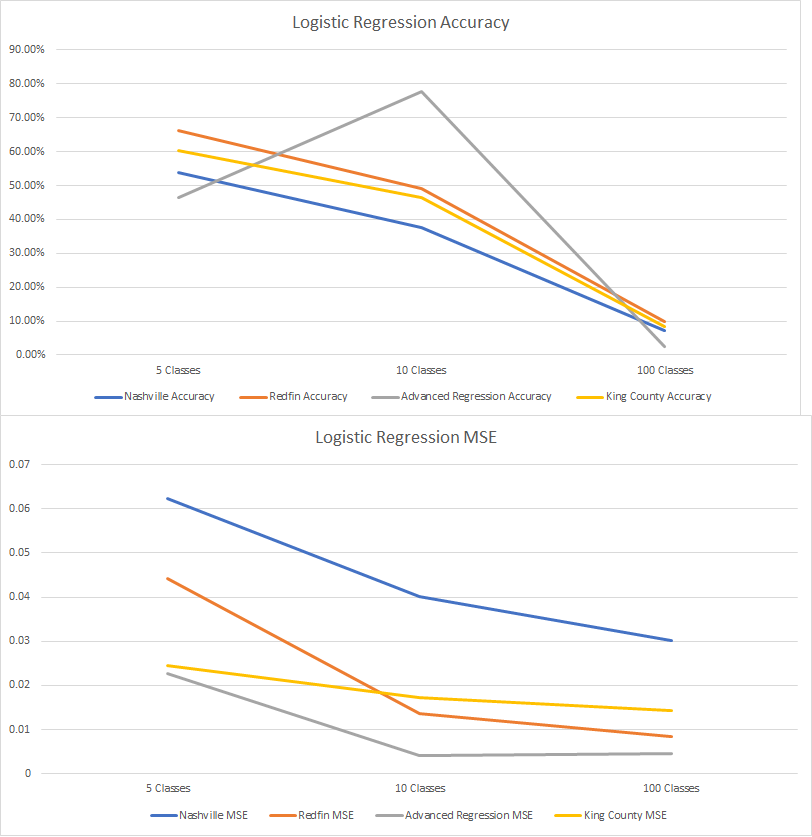
\includegraphics[scale=0.6]{Images/LogisticRegressionMSEAccuracy} \\
			\captionof{figure}{MSE and accuracy for Logistic Regression.}
			\label{fig:logr_MSE_Accuracy}
		\end{center}
			
		\subsection{Decision Tree}
		For our Decision Tree approach, we used a Classification Decision Tree and a Regression Decision Tree. For the Classification Tree, since the data was not already classified, it was split into \(k\) equally sized classes where each class represents a range of prices. The average value for every feature column is also calculated and used to subsitute for any missing data points in the observations. A classification model was built for the King County, Grand Rapids, and Nashville datasets. For each dataset, initially a classification tree model was built using crossfold validation with 10 folds using 90\% of the data for training. This model used the default parameters for tree size, which are maximum number of splits of n-1, minimum leaf size of 1, and minimum parent size of 1. 

		Another classification model was built by using 10 fold cross validation and generating trees for many possible parameters and choosing the model that provides the best training MSE, again using 90\% of the data for training. The results comparing these two models and their training and testing MSEs for the Nashville dataset is shown in Table \ref{table:ctree_performance} below. The MSE indicates the averae squared distance between the predicted class and the actual class, where the classes are represented by a range of integers from 1 to \(k\). In the results below, the number of classes that are being classified is 8.

		\begin{center}
		\captionsetup{type=table}
			\begin{tabular}{l|c}
				Classification Tree Mdodel	& MSE \\
				\hline
				CTree Train Error 			& 0.5225 \\
				CTree Test Error			& 0.6964 \\
				Optimized CTree Train Error & 0.6141 \\
				Optimized CTree Test Error	& 0.6918 \\
			\end{tabular}
			\captionof{table}{Observations from Classification Tree models.}
			\label{table:ctree_performance}        
		\end{center}

		For the Classification Tree, the optimized parameters result in much higher testing error, but also a much better testing error. This seems to indicate that default parameters with crossfold validation result in slight overfitting compared to crossfold validation with the optimized parameters.

		Regression Tree models were generated following a similar pattern, creating one 10 fold cross validation Regression Tree model for each dataset using default parameters and creating another Regression Tree model by varying the tree parameters to find the best MSE training error. Table \ref{table:rtree_performance} below shows a table of the MSE results for the Regression Tree approach on the Nashville dataset. 

		\begin{center}
		\captionsetup{type=table}
			\begin{tabular}{l|c}
				Regression Tree Model & MSE \\
				\hline
				RTree Train Error & 13.4e-3 \\
				RTree Test Error & 17.5e-3 \\
				Optimized RTree Train Error & 15.1e-3 \\
				Optimized RTree Test Error & 16.8e-3 \\
			\end{tabular}
			\captionof{table}{Observations from Regression Tree models.}
			\label{table:rtree_performance}        
		\end{center}
	
		The Regression models perform similarly, with slightly better results using the optimized parameters for the regression tree compared to the default parameters. The next step in the project is to see how Random Forest ensembles will perform compared to these single highly optimized trees.

		For Random Forest generation, bootstrap replication was used to generate training sets for each tree. For training, 70\% of each data set was used for training, and n random samples were taken with replacement, where n is the size of each training set. For the decision tree creation, each split decision chose amoung a random subset of m features. Different Random Forest models were tested using various numbers of features. Random Forests were tested with 5\% of features sampled, 15\% of features sampled, 30\% of features sampled, 45\% of features sampled, 60\% of features sampled, 75\% of features sampled, and square root of m features sampled. Random Forests were also grown with different number of trees to see how the number of trees affected performance. Forests with 50 trees, 100 trees, and 500 trees were tested. None of the trees were pruned, and a few tests were done to see how limiting growth of the trees would affect results. 

		The team's expectations for the Random Forest parameters were that more trees would result in better testing error rates, with a limit where the number of trees stops changing performance, and that smaller feature sample numbers would result in the best results. The more trees that are added, the more each tree's tendency to overfit would be averaged out, and the smaller feature sample numbers would reduce variance from noisy parameters, especially in the Nashville dataset, which had the most holes in the data. It was also expected that limiting the sizes of the trees would reduce each tree's tendency to overfit and produce better results as well. 

		The results of this experiment were somewhat mixed. For regression forests, models were created using 50 trees, 100 trees, and 500 trees. For each number of trees, a model was created random sampling 7 different ratios of features, as described above. The performance across these seven were averaged together so that the average performance for each number of trees could be measured as seen in Figure \ref{fig:r_forest_treenum_perf} below. Variance in MSE between 50 trees and 100 trees was minimal. Variance in MSE between 100 trees and 500 trees, however, was more signficant, with the 500 tree models yielding the best individual scores by single feature selection ratio and data set. The results for classification forests were a little more mixed. The averages were taken the same way and can be seen in Figure \ref{fig:r_forest_treenum_perf}, and the performance is more varied with no clear correlation between better results and more trees used. We think this may show that the classifier are more variable depending on the quality of the data and the number of different classes. In this case, the data was divided into eight classes. 

		\begin{center}
		\captionsetup{type=figure}
			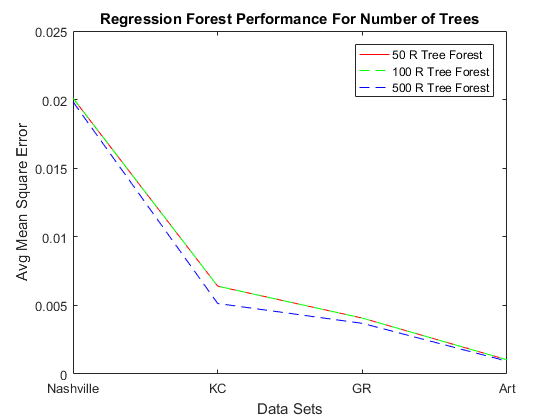
\includegraphics[scale=0.6]{Images/RegressionGraphPerformanceForNumberOfTrees} \\
			\captionof{figure}{Regression Forest Performance for Number of Trees}
			\label{fig:r_forest_treenum_perf}
		\end{center}

		\begin{center}
		\captionsetup{type=figure}
			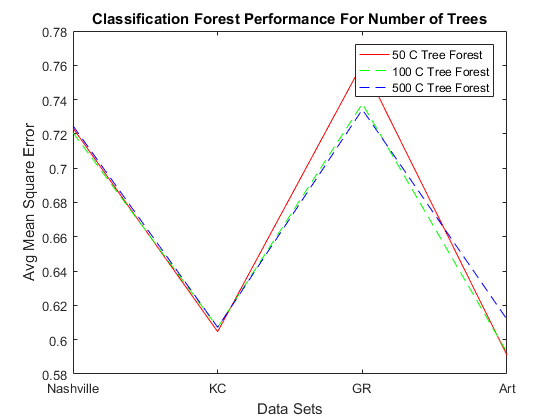
\includegraphics[scale=0.6]{Images/ClassificationGraphPerformanceForNumberOfTrees} \\
			\captionof{figure}{Regression Forest Performance for Number of Trees}
			\label{fig:c_forest_treenum_perf}
		\end{center}

		In terms of the best number of features to randomly sample from during forest generation, the results were not quite as the team expected either. For regression, a few of the data sets worked best with smaller feature samples. But for classification, the amount of features to sample was higher, and there wasn't too much consistency between what sample sizes worked best. The results can be seen in Table \ref{table:best_feature_sample_counts} below, which shows the number of features to randomly sample that worked best for a 500 tree classification and regression forest for each data set, where m is the total number of features in that data set. 

		\begin{center}
		\captionsetup{type=table}
			\begin{tabular}{r|c|c}
				& \small{Regression} & \small{Classification} \\
				\hline
				\small{Nashville Data} & \small{$\floor{\sqrt(m)}$} & \small{$\floor{m \times .60}$} \\
				\hline
				\small{King's County Data} & \small{$\floor{m \times .75}$} & \small{$\floor{m \times .60}$} \\
				\hline
				\small{Grand Rapids Data} & \small{$\floor{m \times .30}$} & \small{$\floor{m \times .60}$} \\
				\hline
				\small{Advanced Reg Data} & \small{$\floor{m \times .30}$} & \small{$\floor{m \times .45}$} \\
				\hline
			\end{tabular}
			\captionof{table}{Best number of features to randomly sample in a Random Forest.}
			\label{table:best_feature_sample_counts}        
		\end{center}

		The performance of the Random Forests compared to single trees also showed some unexpected results. As a control comparison, Random Forests were also grown using MatLab's built in TreeBagger function and used with similar settings. The team's implementation of the Regression Random Forest had slight improvements for two of the data sets, but were very close to how MatLab's random forest performed. But compared to our single regression tree tests, the random forest was not an improvement across the board as expected. In particular, a regression tree with no optimization and a regression tree with optimization both out performed the random forest for the Nashville data set. The team thinks that this may be due to the noise introduced to the Nashville data set when filling in gaps in observations. However, the Grand Rapids data also performed slightly better in the single regression trees than the random forests, and the Grand Rapids data was more complete, so there are other factors that are more uncertain in determining how well the models under or overfit the datasets. The performance of all the regression decision classifers are shown below in Figure \ref{fig:fig_reg_best}.

		\begin{center}
		\captionsetup{type=figure}
			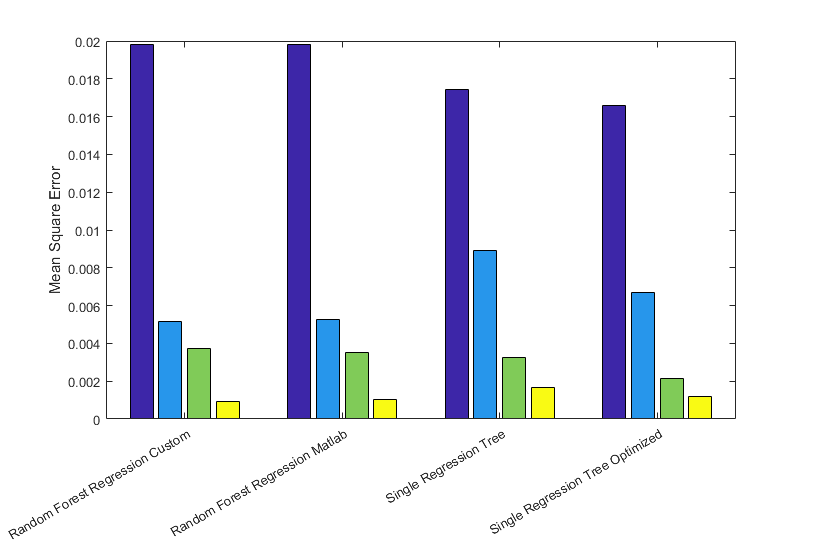
\includegraphics[scale=0.40]{Images/RegressionResults} \\
			\captionof{figure}{Comparison of performances for all decision regression models.}
			\label{fig:fig_reg_best}
		\end{center}

		But again, the results for classification and for regression do not show the same tendencies. The team's implementation of a Classification Random Forest had almost the same performance as a single classification tree. However, MatLab's TreeBagger function creates a significantly better Random Forest Classifier. The team thinks that there may be some details for classification that MatLab implements that the team did not account for, resulting in our performance not showing much improvement. The performance of all classifier decision trees is shown below in Figure \ref{fig:fig_class_best}.

		\begin{center}
		\captionsetup{type=figure}
			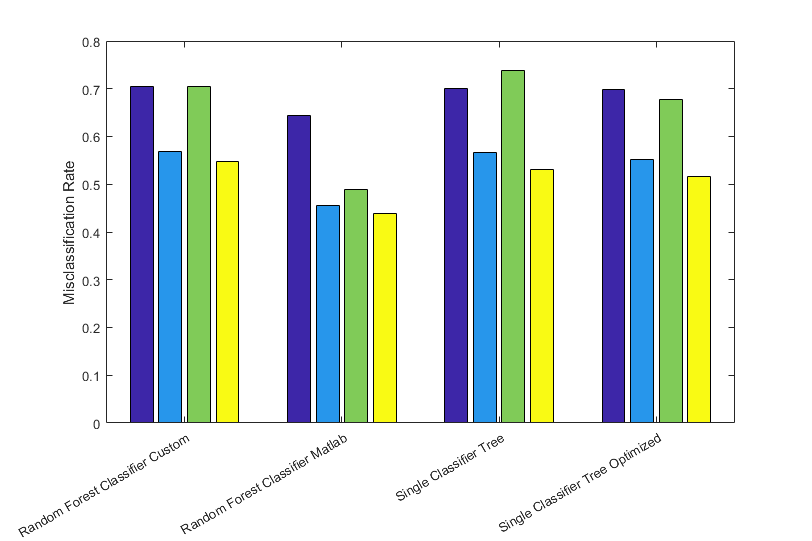
\includegraphics[scale=0.40]{Images/ClassificationResults} \\
			\captionof{figure}{Comparison of performances for all decision classification models.}
			\label{fig:fig_class_best}
		\end{center}

		One trend that can be seen in most of the comparisons is that the Nashville data set, as epxected due to holes in the observations, fairly consistently performs the worst. The primary exception is in the case of a Single Classification Tree seen above, in which the Grand Rapids data set results in a worse model than the Nashville data set. On a similar trend, the Advanced Regression Techniques data met expectations in terms of performing extremely well. It had very low error for the regression trees and performed the best on every single decision tree based model. Another trend noticed with the random forests was training time. The team's implementation of random forest could take several minutes to generate a tree of 100+ forests. MatLab's implementation was a little faster, but still on the order of minutes to train one model on one data set. And a program to test different feature sample sizes and tree sizes for each data set can take hours.  
		
		We also used the Random Forest Models to get an idea of what the most important features are by adding weights to the features that are selected the most often. Figures \ref{fig:r_best_features} and \ref{fig:c_best_features} show the results for this analysis on the Nashville data set, which fell somewhat in the middle for number of features in the data sets. 

		\begin{center}
		\captionsetup{type=figure}
			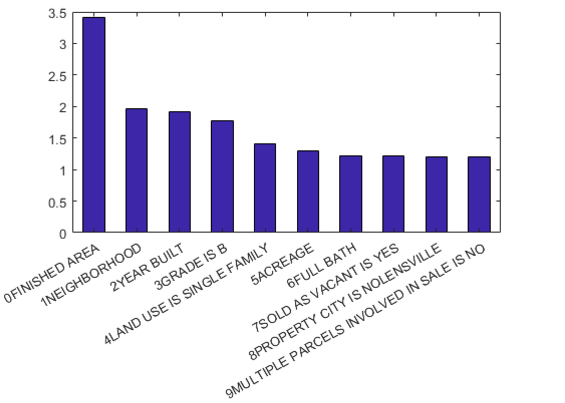
\includegraphics[scale=0.60]{Images/BestFeaturesRegression} \\
			\captionof{figure}{Most sampled features in Regression Forest for Nashville.}
			\label{fig:r_best_features}
		\end{center}

		\begin{center}
		\captionsetup{type=figure}
			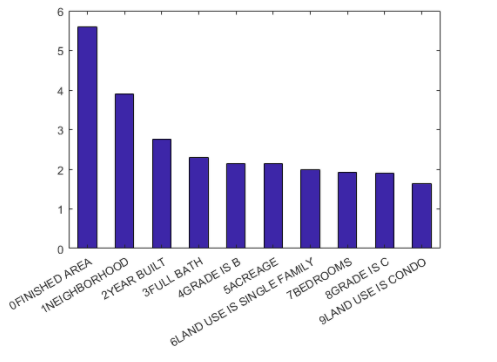
\includegraphics[scale=0.60]{Images/BestFeaturesClassification} \\
			\captionof{figure}{Most sampled features in Classification Forest for Nashville.}
			\label{fig:c_best_features}
		\end{center}

		This can be used to decide if some features should be removed if they are almost never used or setting a threshold to only use features above a certain weight. Knowing the most important factors can also be useful for helping realtors and appraisers give recommendations. But getting the feature weights should be considered against the highly increased training time of a forest versus a single tree. Feature weights could be obtained from a single tree, but those weights are more likely to be skewed by the overfitting tendencies of a single tree. 

		\subsection{Neural Network}

		To compare the other models considered to a deep learning technique, a simple Feedforward Neural Network (FNN) has been implemented with three hidden fully-connected layers. Implementations of this neural network framework have been created in both Python and Matlab\textsuperscript{\cite{git_repo}}. No existing packages or libraries were used outside of basic Python modules, including Numpy for numerical operations. The results obtained for this section are strictly observed from the Python version.
		
		Figure \ref{fig:fig_nn_model} illustrates the architecture of the network. Each layer has its own activation function. In this case, a sigmoid function is used, since all values are normalized within the range of \([0, 1]\). Each data point is considered to have \(d\) features extracted from the data. From the input layer, each data feature's value is sent to every unit in the first hidden layer. From there, the output of each unit is sent as input to each unit in the following layer, until the output layer is reached. The output layer only contains one unit, representing the prediction of the FNN model. In this case, the output is a prediction of the sales price for the housing data features provided to the input layer.
		
		\begin{center}
            \captionsetup{type=figure}
			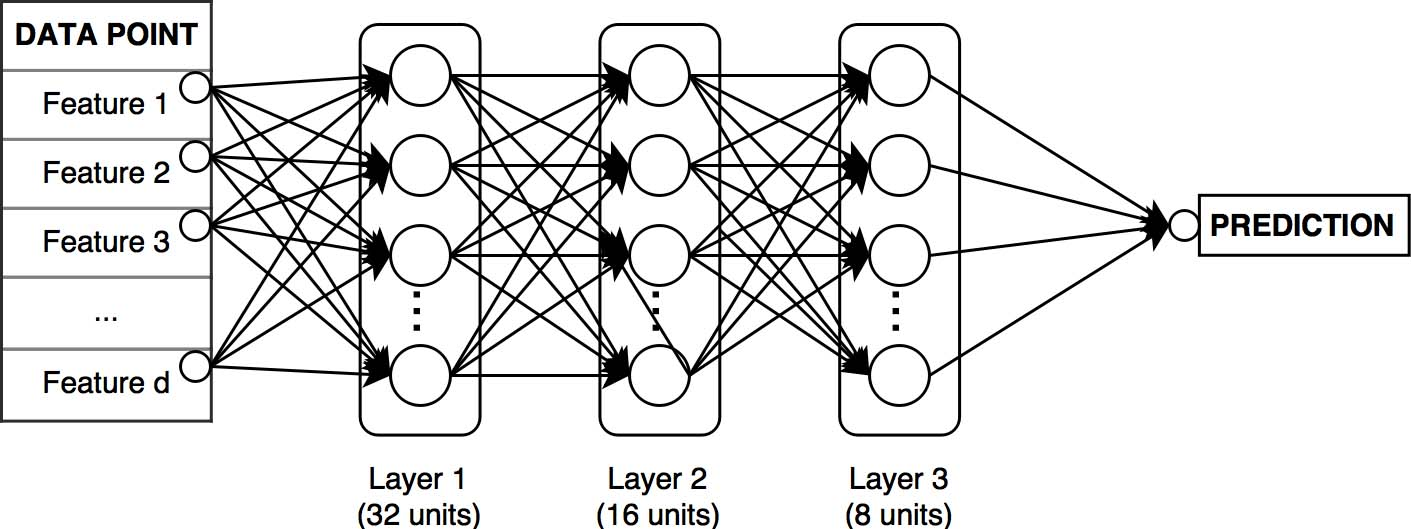
\includegraphics[scale=0.15]{NeuralNet/fig_nn_01} \\
			\captionof{figure}{Architecture of our network.}
			\label{fig:fig_nn_model}
		\end{center}
	
		This network can be represented by the following equations, where \(X\) is the set of data features, \(h\) is the hidden value, \(W\) is a weight matrix for each layer, \(b\) is a bias vector for each layer, and \(y\) is the output prediction from the FNN model.
		\begin{align}
			h_{0} &= X \nonumber \\
			h_{i} &= \sigma(W_{i}h_{i-1} + b_{i}) \nonumber \\
			y &= h_{n} \nonumber
		\end{align}
	
		Performing cross-validation, it was found that using 32 units in the first hidden layer, 16 in the second, and 8 in the third gave ideal performance results.
		
		Input data is randomly shuffled and split into training and testing datasets, with a ratio of \(2:1\). To optimize the network's weights after each iteration of training, three different gradient descent methods are considered: Stochastic Gradient Descent, an Adaptive Gradient Descent (Adagrad) \textsuperscript{\cite{nn_adagrad}}, and an Adaptive Learning Rate (Adadelta) method \textsuperscript{\cite{nn_adadelta}}. The version of SGD considered included a momentum in the following form:
		\begin{align}
			v &= \gamma v + \eta \nabla W \nonumber \\
			\Delta W &= -v \tag{SGD w/ momentum}
			\intertext{where \(\Delta W\) is the change in weight, \(\nabla W\) is the computed gradient from a batch of training data, \(v\) is a velocity term, \(\gamma\) is a momentum hyperparameter, and \(\eta\) is a learning rate hyperparameter.} \nonumber
		\end{align}
		Adagrad extends upon this by also considering an accumulation of the sum of squared gradients over time.
		\begin{align}
			\Delta W &= -\frac{\eta}{\sum{\nabla W...}}\nabla W \tag{Adagrad}
		\end{align}
		This modification allows for a sort of adaptive behavior, where the step size decreases as the gradient descent method approaches a minima. The Adadelta method takes this one step further and instead of considering the sum of all squared gradients equally, those gradients measured more recently have more influence on each weight update. Specifically, this modifies the change in weights as follows.
		\begin{align}
			\Delta W &= -\frac{\text{RMS}(\Delta W...)}{\text{RMS}(\nabla W...)}\nabla W \tag{Adadelta} \\
			\intertext{where \(\text{RMS}(\Delta W...)\) is the Root Mean Squared of the past weight changes, and \(\text{RMS}(\nabla W...)\) is the Root Mean Square of the past gradients measured.} \nonumber
		\end{align}
		Figures \ref{fig:fig_nn_result1}, \ref{fig:fig_nn_result2}, \ref{fig:fig_nn_result3}, and \ref{fig:fig_nn_result4} show our observations from using all three gradient descent methods on each dataset. With the exception of the ART dataset, it can be seen that after training for 300 iterations, Adadelta outperforms Adagrad, and Adagrad outperforms SGD. It should be noted that the hyperparameters used for these results are \(\eta=0.1\) and \(\gamma=0.9\). These values were chosen after a running a series of trials for cross-validation.

		Table \ref{table:nn_performance} includes the final loss values computed for each dataset, measured as MSE. Generalized performance was observed to be far greater on the ART dataset than any other.

		\begin{center}
			\captionsetup{type=figure}
			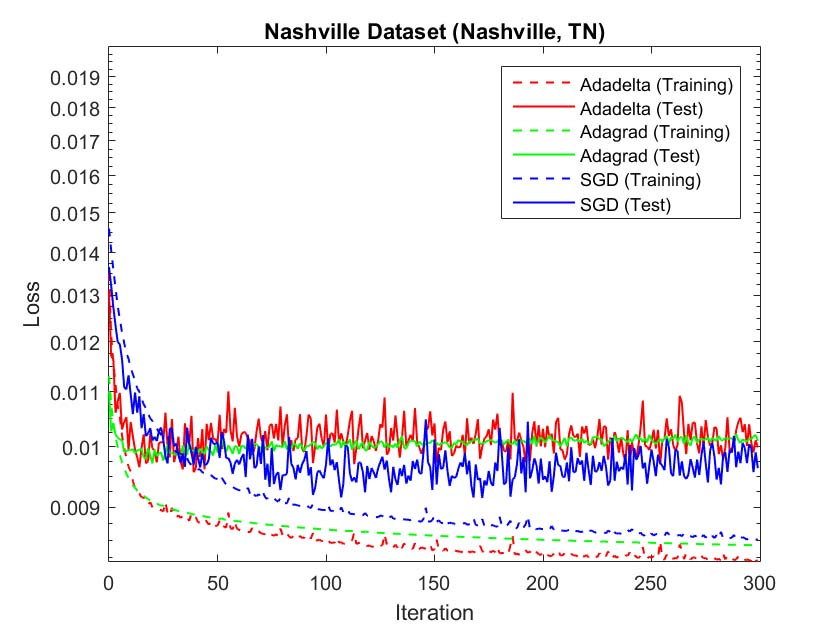
\includegraphics[scale=0.27]{NeuralNet/fig_nn_05} \\
			\captionof{figure}{MSE of FFN on Nashville dataset.}
			\label{fig:fig_nn_result4}
		\end{center}

		\begin{center}
            \captionsetup{type=figure}
			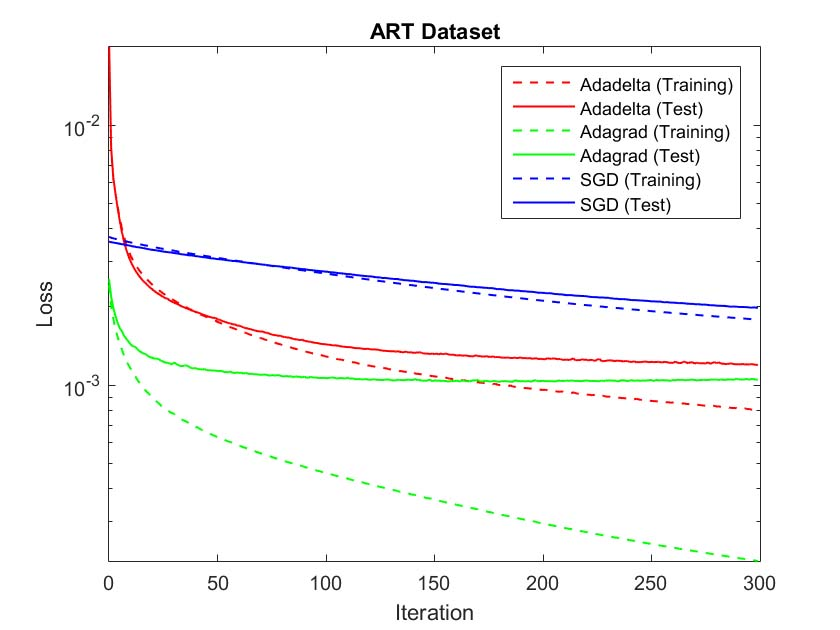
\includegraphics[scale=0.27]{NeuralNet/fig_nn_02} \\
			\captionof{figure}{MSE of FFN on ART dataset.}
			\label{fig:fig_nn_result1}
		\end{center}

		\begin{center}
			\captionsetup{type=figure}
			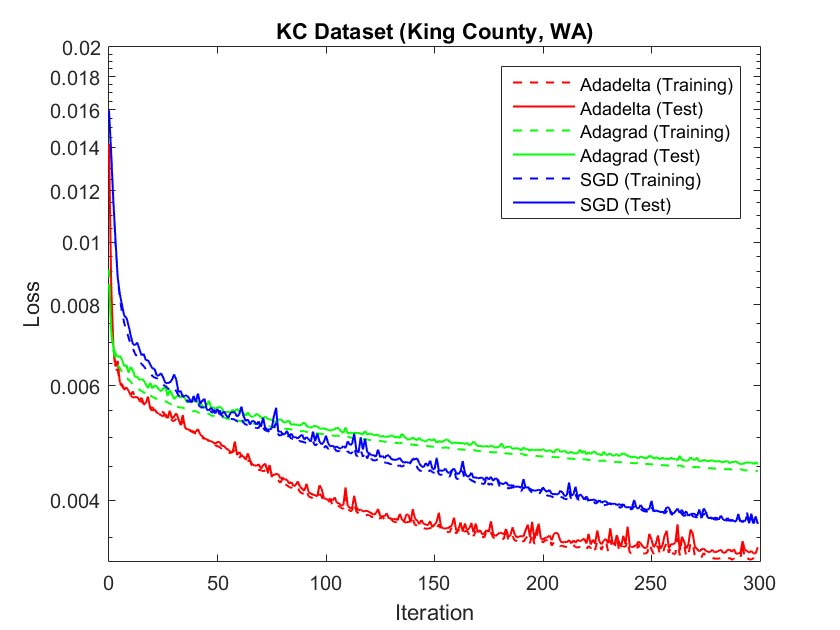
\includegraphics[scale=0.27]{NeuralNet/fig_nn_04} \\
			\captionof{figure}{MSE of FFN on King County dataset.}
			\label{fig:fig_nn_result3}
		\end{center}
	
		\begin{center}
            \captionsetup{type=figure}
			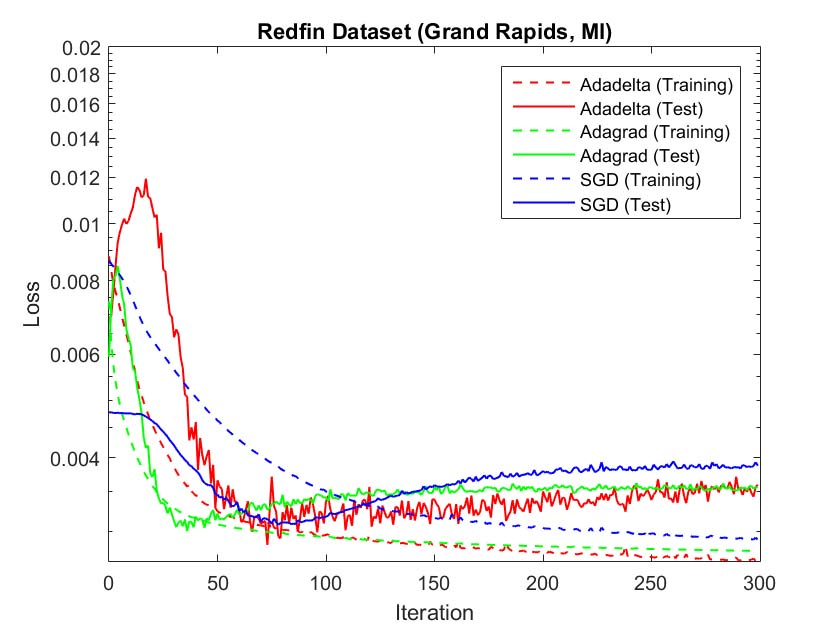
\includegraphics[scale=0.27]{NeuralNet/fig_nn_03} \\
			\captionof{figure}{MSE of FFN on Grand Rapids dataset.}
			\label{fig:fig_nn_result2}
		\end{center}
	
		\begin{center}
			\captionsetup{type=table}
			\begin{tabular}{l|c|c|c}
				& \multicolumn{3}{c}{Loss (MSE)} \\
				Dataset 		& SGD		& Adagrad	& Adadelta \\
				\hline
				Nashville 		& 9.6e-3 	& 10.1e-3 	& 9.9e-3 \\
				ART 			& 1.9e-3 	& 1.1e-3 	& 1.2e-3 \\
				King County 	& 3.7e-3 	& 4.5e-3 	& 3.3e-3 \\
				Grand Rapids 	& 3.8e-3 	& 3.5e-3 	& 3.6e-3 \\
			\end{tabular}
			\captionof{table}{Observed generalized performance from FNN.}
			\label{table:nn_performance}
		\end{center}
	
		Aside from measuring error in the FNN model's predictions as MSE, an accuracy measure was also computed, where predictions are considered correct if they fall within \(\pm\)\$10k from the true sales price. The observed accuracies of the model on each dataset are shown in Table \ref{table:nn_accuracy}.
		
		\begin{center}
		\captionsetup{type=table}
		\begin{tabular}{l|c|c|c}
			& \multicolumn{3}{c}{Accuracy (within \(\pm\)\$10k)} \\
			Dataset 		& SGD			& Adagrad		& Adadelta \\
			\hline
			Nashville		& \(9.1\%\)		& \(9.3\%\)		& \(10.0\%\) \\
			ART 			& \(19.5\%\) 	& \(25.8\%\)	& \(24.0\%\) \\
			King County 	& \(12.1\%\) 	& \(11.5\%\)	& \(13.7\%\) \\
			Grand Rapids 	& \(10.6\%\) 	& \(11.2\%\)	& \(13.5\%\) \\
		\end{tabular}
		\captionof{table}{Observed generalized accuracy from FNN.}
		\label{table:nn_accuracy}
		\end{center}
		
		The accuracy observed from this model leaves much to be desired, but it is assumed that weak performance is due to a limited amount of quality data, or rather stronger performance could be obtained from a training dataset that is more balanced and representative of the general population of data. Better performance can be found on the ART dataset, which came complete, requiring no substitution of missing values. Furthermore, the ART dataset covered a more consistent range of sales prices, whereas the other datasets had large gaps in both data features and ranges of sales prices. Another conclusion that can be drawn is simply from the features provided by each dataset. Obviously, more meaningful information could be drawn from those features found in the ART dataset. In any case, for all four datasets, the FNN model demonstrates an ability to learn some information about the sales prices of each house, and its results are comparable if not better than the other models we consider.
		
 		\section{Conclusion}
 		Our goal has been to observe the effectiveness of different machine learning approaches to the problem of real estate valuation. A variety of models have been implemented, to include linear regression, logistic regression, decision trees, neural networks, and ensemble methods. These approaches have provided some interesting comparisons, but one consistent observation has been that all models are greatly affected by the quality of data given.

		First, processing the data for use by the models is extremely necessary. This includes filtering and transforming the data into a format that any the model can handle well, such as splitting categorical features up into binary categories. Additionally, filling in gaps of missing data can significantly improve a model's ability to predict or classify.

		Ultimately, while there are things that can be done to extract meaningful information, a machine learning model is limited by how much information is actually in the data.  Table \ref{table:results} shows the generalized performance of our implementation for each model.  In all cases, the models performed best on the ART dataset.  This data is both complete and has the largest number of features.  In contrast, the Nashville dataset performs the worst, due to have the largest gaps in data. Given more feature-rich and complete housing data would certainly improve the performance of all models considered.
		
		\begin{center}
	        \captionsetup{type=table}
	        \begin{tabular}{l|c|c|c|c}
	        	         & Nash.   & ART     & Kng Cty & Gr Rpds \\
	        	\hline
	        	Lin Reg  & 22.1e-3 & 1.0e-3  & 13.1e-3  & 6.3e-3 \\
	        	Lin Ens  & ---     & 1.8e-3  & 13.1e-3  & 5.1e-3 \\
	        	Log Reg  & ---     & 4.5e-3  & 14.4e-3  & 8.5e-3 \\
	        	Log Ens  & ---     & 1.7e-3 & 13.2e-3  & 8.1e-3 \\
	        	RTree  	 & 16.6e-3 & 1.2e-3	 & 6.7e-3  & 2.2e-3  \\
	        	Ran Frst & 19.8e-3 & 0.9e-3  & 5.1e-3  & 3.7e-3  \\
	        	FNN      & 9.6e-3  & 1.1e-3  & 3.3e-3  & 3.5e-3  \\	        	
	        \end{tabular}
			\captionof{table}{MSE observed from all models.}
			\label{table:results}
		\end{center}
		\begin{thebibliography}{13}
			\bibitem{nashville_data}
			\textit{Nashville Housing Data: Home value data for the booming Nashville Market}
			Retrieved from \\ \small{\url{https://www.kaggle.com/tmthyjames/nashville-housing-data/}}
			
			\bibitem{kc_data}
			\textit{House Sales in King County, USA: Predict house price using regression}
			Retrieved from \\ \small{\url{https://www.kaggle.com/harlfoxem/housesalesprediction}}	
			
			\bibitem{kaggleblog}
			\textit{Data-driven property valuations: the real deal?}
			Retrieved from \\ \small{\url{http://blog.kaggle.com/2010/06/21/data-inc-are-avms-soothsayers-or-the-real-deal/}}
			
			\bibitem{scotsman}
			Schroeder, Steve.
			\textit{Fighting Fraud: A combination of collateral assessment and AVMs can maximize mortgage-fraud management}
			Retrieved from \\ \small{\url{http://www.scotsmanguide.com/Residential/Articles/2005/10/Fighting-Fraud/}}
			
			\bibitem{zillow}
			\textit{What is a Zestimate? Zillow's Home Value Forecast.}
			Retrieved from \\
			\small{\url{http://www.zillow.com/zestimate/}}
			
			\bibitem{lowrance}
			Lowrance, R. E. (2015).
			\textit{Predicting the Market Value of Single-Family Residential Real Estate}
			(Doctoral Dissertation). New York University. Retrieved from \small{\url{http://gradworks.umi.com/36/85/3685886.html}}
			
			\bibitem{park}
			Park, B., \& Bae, J. K. (2015).
			\textit{Using machine learning algorithms for housing price prediction: The case of Fairfax County, Virginia housing data.}
			Expert Systems with Applications, 42(6), 2928-2934. doi:10.1016/j.eswa.2014.11.040
			
			\bibitem{bin} 
			Bin, O. (2004).
			\textit{A prediction comparison of housing sales prices by parametric versus semi-parametric regressions.}
			Journal of Housing Economics, 13(1), 68-84. doi:10.1016/j.jhe.2004.01.001
			
			\bibitem{bourassa1} 
			Bourassa, S. C., Cantoni, E., \& Hoesli, M. (2010). 
			\textit{Predicting House Prices with Spatial Dependence: Impacts of Alternative Submarket Definitions.}
			SSRN Electronic Journal. doi:10.2139/ssrn.1090147
			
			\bibitem{bourassa2}
			Bourassa, S. C., Cantoni, E., \& Hoesli, M. (2007).
			\textit{Spatial Dependence, Housing Submarkets, and House Prices.}
			SSRN Electronic Journal. doi:10.2139/ssrn.771867
			
			\bibitem{kauko}
			Kauko, T., Hooimeijer, P., \& Hakfoort, J. (2002).
			\textit{Capturing Housing Market Segmentation: An Alternative Approach based on Neural Network Modelling.}
			Housing Studies, 17(6), 875-894. doi:10.1080/02673030215999
			
			\bibitem{azadeh} 
			Azadeh, A., Ziaei, B., \& Moghaddam, M. (2012).
			\textit{A hybrid fuzzy regression-fuzzy cognitive map algorithm for forecasting and optimization of housing market fluctuations.}
			Expert Systems with Applications, 39(1), 298-315. doi:10.1016/j.eswa.2011.07.020
			
			\bibitem{fan}
			Fan, G., Ong, S. E., \& Koh, H. C. (2006).
			\textit{Determinants of House Price: A Decision Tree Approach.}
			Urban Studies, 43(12), 2301-2315. doi:10.1080/00420980600990928
			
			\bibitem{nn_adagrad}
			Duchi, J., Hazan, E., \& Singer, Y. (2011). \textit{Adaptive Subgradient Methods for Online Learning and Stochastic Optimization}. Journal of Machine Learning Research.
			
			\bibitem{nn_adadelta}
			Zeiler, M. \textit{Adadelta: An Adaptive Learning Rate Method}. arXiv:1212.5701v1
			
			\bibitem{git_repo}
			\url{https://github.com/msu-ml/17spr_lingg_langford_lucero.git}
		\end{thebibliography}
	\end{multicols}
\end{document}
